\documentclass[reprint,english,notitlepage]{revtex4-2}
\usepackage{amsmath}
\usepackage[mathletters]{ucs}
\usepackage[utf8x]{inputenc}
\usepackage[english]{babel}
\usepackage{esint}
\usepackage{physics,amssymb}
\usepackage{graphicx}
\usepackage{xcolor}
\usepackage{hyperref}
\usepackage{listings}
\usepackage{subfigure}
% \usepackage{biblatex}
% \usepackage[style=science, backend=biber]{biblatex}
% \addbibresource{References_Part_4.bib} TODO: Slett før innlevering
\hypersetup{
    colorlinks,
    linkcolor={red!50!black},
    citecolor={blue!50!black},
    urlcolor={blue!80!black}}

\lstset{inputpath=,
    backgroundcolor=\color{white!88!black},
    basicstyle={\ttfamily\scriptsize},
    commentstyle=\color{magenta},
    language=Python,
    morekeywords={True,False},
    tabsize=4,
    stringstyle=\color{green!55!black},
    frame=single,
    keywordstyle=\color{blue},
    showstringspaces=false,
    columns=fullflexible,
    keepspaces=true}

\begin{document}

\title{}
\author{Oskar Idland \& Jannik Eschler}
\date{\today}
\affiliation{Institute of Theoretical Astrophysics, University of Oslo}

\begin{abstract}
    This is an abstract \colorbox{red}{Complete this summary at the end of the paper}
\end{abstract}
\maketitle
\section{Introduction} \label{sec: introduction}
In this text we are going to explore our very own star and compare it to another known star named the Sun. This will teach you how one can extract valuable information about a star's physical properties, its birth, life and death. Lets begin by looking at our star in its current state      

\section{Our star: Its current state and origin}
\subsection{The main sequence}
\begin{figure}[h!]
  \centering
  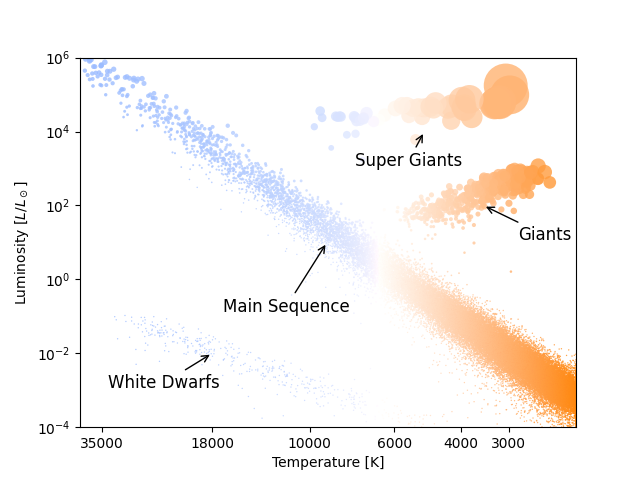
\includegraphics[scale = .50]{figures/HR-Diagram_Classification.pdf}
  \caption{HR-Diagram}
  \label{fig: HR_diagram}
\end{figure}
In Figure \ref{fig: HR_diagram} you can see what is called and HR-diagram. This is a way to portray the behavior of most stars in their life cycle. The x-axis is the surface temperature of the star, and the y-axis is the luminosity as fraction of the Sun's luminosity. In Figure \ref{fig: HR_diagram_The_Sun} you see the Sun's placement in the diagram in its true size relative to other stars. The diagonal strip it occupies is known as the "The Main Sequence" and is where most stars spends most of their life. 

\begin{figure}[h!]
  \centering
  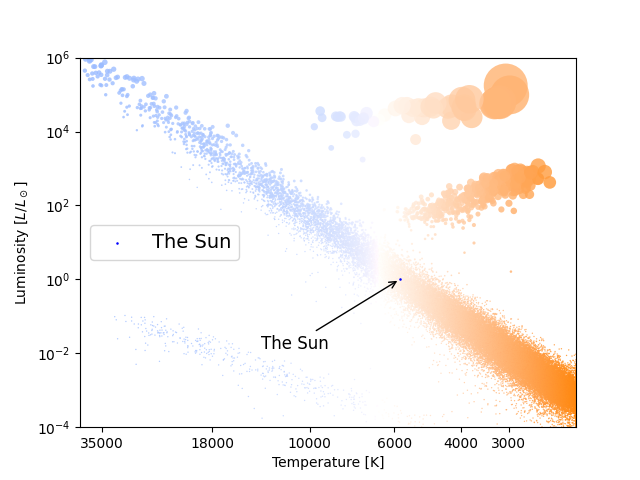
\includegraphics[scale = .5]{figures/HR_diagram_The Sun.pdf}
  \caption{The Sun in the HR-Diagram}
  \label{fig: HR_diagram_The_Sun}
\end{figure}

\subsubsection*{The Placement of Our Star}
To find our star's position we need both its temperature and luminosity. From earlier measurement we know our star has a surface temperature $ T $ of 11733 Kelvin. Luminosity is defined as energy per unit of time. 
\begin{equation} \label{eq: Luminosity}
  L = \frac{E}{dt}
\end{equation}  

Flux is defined as energy per unit of area per unit of time. 
\begin{equation} \label{eq: Flux}
  F = \frac{E}{dAdt}
\end{equation}

We can use this to find a new way to express the Luminosity. 
\begin{equation} \label{eq: Lumin 2}
  L = FdA 
\end{equation}
Stefan-Boltzmann's law%~\parencite[][p. 3]{for_notat_3d} TODO: Remove Comment
dictates that the flux $ F $ can be expressed as

\begin{equation}\label{eq: Flux 2}
  F = σT^{4}.
\end{equation}

Where $ T $ is the temperature in Kelvin and $ \sigma  $ is Stefan-Boltzmann's constant. We also know the total area of a sphere to be $ 4 \pi r^{2} $  where $ r $ is the radius of the sphere. Combining this and equations \ref{eq: Lumin 2} \& \ref{eq: Flux 2} we get the following expression for the luminosity.

\begin{equation} \label{eq: Luminosity final}
  L = σT^{4} 4 π r^{2}
\end{equation}
Using our measured surface temperature of our star we get a luminosity $ L = 5.79 \cdot 10^{28} W$  or $ 1.51 \cdot 10^{2} L_{\odot} $. The use of the  $ "\odot" $ symbol is a way to express a quantity as a fraction of said quantity in relation to the Sun. An example would be $ M_{⊙} $ and $ L_{⊙} $ being the mass and luminosity of the sun respectively. This kind of notation is useful as it creates an easy baseline of comparison of different stars.
Now we have the coordinates needed to plot our star in the HR diagram. 
\begin{figure}[h!]
  \centering
  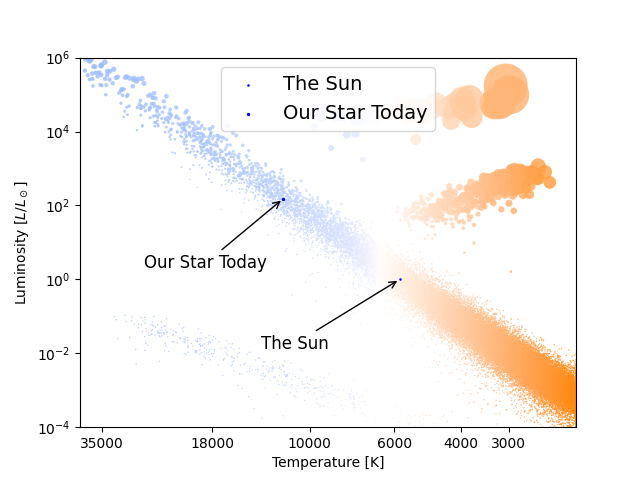
\includegraphics[scale = .5]{figures/HR_diagram_Sun and Star}
  \caption{Our Star and the Sun in the HR-Diagram. Both in true size relative to the other stars}
  \label{fig: HR_Diagram_Today}
\end{figure}
It seems our star is a main sequence star! This was very likely as this is where most stars spends most their time. Speaking of which, lets see how we can determine the lifespan of our star. 

\subsubsection*{The Lifespan of Our Star}
In all stars their is a struggle between two forces. The first being the gravitational force trying to crush all the atoms in the star in on itself. The other being the radiation pressure generated from the fusion of mainly hydrogen inside the star. As more and more hydrogen is turned into helium the mean molecular weight $ μ $ of the star increases and as such, its mass increases as well. When the mass increases the gravitational force increases and the star will shrink. The shrinkage will create higher pressure and temperature which will make the fusion more effective, increasing the radiation pressure. The two forces will balance each other until the star has a relatively stable radius until there isn't enough hydrogen to stop the gravitational forces, but we will cover this later. When these two forces are equal, the star has reached hydrostatic equilibrium. 

This tells us there is a relationship between the mass of the star and its lifetime $ t $. The equation expressing this relationship (derived in %~\parencite[][p. 7]{for_notat_3d}) TODO: Remove Comment
is as follows:
\begin{equation} \label{eq: Lifetime}
  t = \frac{pMc^{2}}{L}
\end{equation}
Where $ p $ is the fraction of the total mass being converted into energy, $ M $ is the mass of the star, $ L $ being the luminosity and $ c $ being the speed of light. We will assume this to be 10\% as this is true for the Sun. Using equation \ref{eq: Lifetime} we get a lifetime of 3.04e+08 years. This is approximately 3\% of the Sun's lifespan!

\subsubsection*{Relationships between mass, temperature and luminosity}
As one can see from the HR-diagram~\ref{fig: HR_diagram}, there is a clear relationship between the temperature and luminosity of a star as they sit on the main sequence.
We therefore expect to see "well behaved" main sequence stars to obey certain ratios.
Derived in%~\parencite[][equation 4]{for_notat_3b} TODO: Remove Comment
we see the two following equations
\begin{equation}\label{eq: T M ratio}
  M ∝ T^{2}_{eff}
\end{equation}
where the mass of a star is proportional to the surface temperature. 
\begin{equation}\label{eq: M L ratio}
  L ∝ M^{4}
\end{equation}
where the luminosity is proportional with the mass. To see if our star is well behaved we will calculate both ratios and compare them with the Sun. 

\begin{center}
  \begin{tabular}{|c|*{2}{c|}}
    \hline
     &M-L Factor  &T-M Factor  \\
    \hline
    The Sun  &4.1 $ ⋅ 10^{94} $ &5.9 $ ⋅ 10^{22} $ \\
    \hline
    Our Star  &1.0 $ ⋅ 10^{95} $ &6.4 $ ⋅ 10^{22} $ \\
    \hline
    \end{tabular}
\end{center}
The T-M factor of both stars are quite close and have the same order of magnitude. With a mass $ M $ of about $ 4.4 M_{⊙} $ its not surprising to see our M-L factor being a bit higher. Although barely one order of magnitude higher. One could say our star is quite well behaved. 

\subsection{Giant Molecular Cloud}
Star do not begin their existence as bright, hot spheres creating fusion reaction at a scale we could only dream of on earth. Instead, they start their life as cold Giant Molecular Clouds (GMC) of different gases. For a star to form there need to be a strong enough gravitational pull to overpower the gas pressure. As a consequence, there is a maximum radius this cloud can have for it to collapse in on itself. We cannot go back in time to see what our star looked like before it was born, but we can make an educated guess! For this we will assume our GMC has:
\begin{itemize}
  \item The same mass as our star today
  \item Collapsed in on itself without external forced like a supernova
  \item Is spherically symmetrical
  \item Has a temperature of 10 K
  \item Is made up of 75\% Hydrogen and 25\% Helium
\end{itemize} 
As derived in%~\parencite[][Section 3]{for_notat_3b} TODO: Remove Comment
, there is a minimum radius requirement radius $ R_j $ for a GMC to collapse in on itself.
\begin{equation}
  R_j = \left( \frac{15kT }{4 π G μ m_h ρ} \right) ^{\frac{1}{2}}
\end{equation}
Where $ T $ is the temperature of the cloud, $ k $ is Boltzmann's constant, $ G $ the gravitational constant and $ m_h $ the mass of a hydrogen atom. $ μ $ is the mean molecular weight of the cloud which in our case is $ μ = 1.74 $. We replace the density $ ρ $ with the mass $ M $ divided by the volume $ V = \frac{4}{3} π r^{3} $. This gives us the new expression we will use to calculate the smallest possible radius our GMC could have had. 
\begin{equation}\label{eq: Jeans length}
  R = \frac{GMμ m_h }{5kT} 
\end{equation}
Using the mass of our star we get a Jean's Length $ R_j $ of 7.5e+15 meters. To see how big this is in comparison with other stars lets place it into the HR-Diagram! Before we can do this we need to find its luminosity. We already have its radius and temperature so we will use equation \ref{eq: Luminosity final} again. 
\begin{equation}
  L_{\text{GMC}} = 1.1 ⋅ 10^{2}\ L_{⊙}
\end{equation}
Now we are finally able to put it in our HR-Diagram! The GMC is at the size of giant stars. 
\begin{figure}[h!]
  \centering
  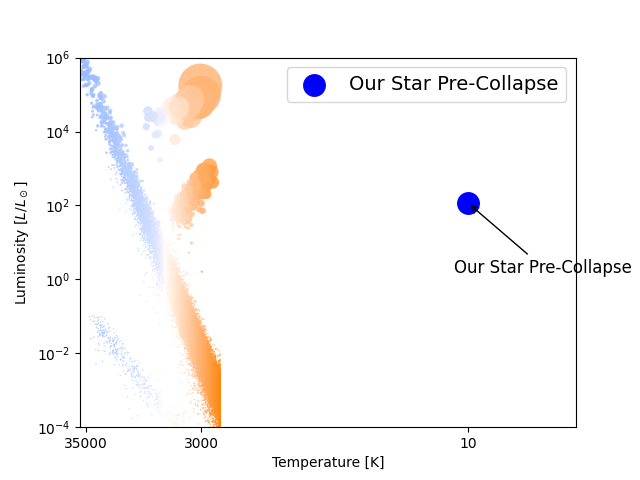
\includegraphics[scale = .5]{figures/HR_diagram_Pre-Collapse}
  \caption{Our star as a GMC plotted true to size}
  \label{fig:figure1}
\end{figure}

\section{Nuclear Reactions in our stars core}
Now we will explore our star internally and take a look at the processes happening on the inside. This will include core temperature, energy production and luminosity. To simplify the problem we will invoke a few assumptions: 
\begin{itemize}
  \item We assume the density of our star is uniform
  \item We will approximate the pressure inside as an ideal gas, not taking other forces such as radiation pressure into account
  \item We will assume hydrostatic equilibrium
  \item We will assume our star consist entirely of protons 
\end{itemize}

\subsection{Core Temparature}
To calculate the core temperature we first need an expression of the mass profile of our star. As when we derived equation \ref{eq: Jeans length} we can express the mass of our star as the following. 
\begin{equation} \label{eq: Mass profile}
  M(r) = ρ_{0} \frac{4}{3} π r^{3}
\end{equation}
As we assume the star to be made up of an ideal gas, the pressure $ P $ will obey the ideal gas law. 
\begin{equation}\label{eq: Ideal gas}
  P = \frac{ρ_{0}kT(r)}{μm_h}
\end{equation}
Since our star is on the main sequence we know it has reach hydrostatic equilibrium. Which let's us describe the change in pressure $ \frac{dP}{dr} $ as a function of radius. 
\begin{equation}\label{eq: hydro equilibrium}
  \frac{dP}{dr } =  - ρ_{0} G \frac{M(r)}{r^{2}} 
\end{equation}
Inserting our equation for the mass profile \ref{eq: Mass profile} into our equation for an ideal gas \ref{eq: hydro equilibrium}, and comparing it with the derivative of our equation for hydrostatic equilibrium we get the following. 
\begin{equation}
  \frac{\mathrm{d}}{\mathrm{d}r} \frac{ρ_{0}kT(r)}{μm_h} = -ρ_{0}^{2}G \frac{4}{3} πr
\end{equation}
We solve this for $ T(r) $. 
\begin{equation} \label{eq: Temp derivative}
  \frac{\mathrm{d}}{\mathrm{d}r}T(r) = - \frac{4 π G ρ_{0}μ m_h r}{3k}
\end{equation}
As the core temperature $ T_c = T(0) $  and we already know the surface temperature $ T(R) $ we want to integrate our equation \ref{eq: Temp derivative} from the core to the surface. 
\begin{equation}
  \int_{0}^{R} \frac{\mathrm{d}}{\mathrm{d}r}T(r) \mathrm{d}r = T(R) - T(0) = - \frac{4 π G ρ_{0}μ m_h R}{3k}
\end{equation}
Replacing $ T(0) $ with $ T_c $, $ T(R) $ with $ T_\text{surface} $ and solving for this we get the following. 
\begin{equation}\label{eq: Core Temp}
  T_c = T_{\text{surface }} + \frac{4 π G ρ_{0}μ m_h R}{3k}
\end{equation} 
As we assumed our star is made op entirely of protons our mean molecular weight $ μ = 1 $. Using our final equation \ref{eq: Core Temp} we get a core temperature $ T_c $ of 17 million Kelvin
\begin{equation}\label{eq: T_c}
  T_c = 1.72 ⋅ 10^{7} K
\end{equation}

\subsection{Energy Production and Luminosity}
We are now going to re-calculate the luminosity of our star based on the nuclear reactions happening in its core. To model these reactions we are going to invoke a few assumptions. 
\begin{itemize}
  \item All nuclear reactions take place within a sphere of 0.2R 
  \item Uniform density
  \item The core temperature temperature is the same throughout the whole sphere
  \item Assume energy production occurs via the pp-chain and CNO-cycle
  \item The core consist of 76.5\% Hydrogen, 25.3\% Helium and 0.2\% Carbon, Oxygen and Nitrogen 
\end{itemize}
As our star has a core temperature $ T_c $ of about 17 million Kelvin the most dominant chain reactions in the core is the pp-chain and the CNO-cycle. The basic equation for calculating energy released per kg per second we get from%~\parencite[][page 4]{for_notat_3c}. TODO Remove Comment
\begin{equation}\label{eq: chain reaction}
  ε_{\text{AB }} = ε_{\text{0, reac}} X_{S} X_{B} ρ^{α} T^{β}
\end{equation}
In this equation, $ \rho $ is the density, $ \alpha $ and $ \beta $ are indices which depend on the temperature $ T $ and $ X_{A} $ and $ X_{B} $ is the mass fraction of the two nuclei in the reaction which follow the following definition.
\[
X_{A} = \frac{n_{A}m_{A}}{nm} = \frac{\text{total mass in type A nuclei}}{\text{total mass}}
\]

The pp-chain is actually multiple chain reactions. We will focus on the the most important one, namely the pp-I chain. This chain reaction converts four $ _{1}^{1}\text{H} $ to $ _{2}^{4}\text{He} $ and is the most efficient at 15 million Kelvin. We will now introduce a new way of writing temperature. With this notation $ T_{n} = T ⋅ 10^{n}K $. This is used in the equation for the pp-chain as follows, derived in%~\parencite[][page 6]{for_notat_3c}. TODO: Remove Comment
\begin{equation}\label{eq: pp-chain}
  ε_{\text{pp}} ≈ ε_{\text{0, pp}}X^{2}_{H}ρ T^{4}_{6}
\end{equation}

In this equation, $ ε_{\text{0, pp}} = 1.08 ⋅ 10^{-12}Wm^{3} / kg^{2} $, the efficiency of the pp-chain is 0.007 meaning only 0.7\% of the mass in each reaction is converted into evergy, $ ρ $ the density of our star, $ X_{H} = 0.745$ and $ T = T_c $ being our star's core temperature calculated in equation \ref{eq: T_c}. Using all this we get a result of 
\begin{equation}\label{eq: E_pp}
  ε_{\text{pp}} ≈ 1.25 ⋅ 10^{-5}
\end{equation}

The CNO-cycle also converts four $ _{1}^{1}\text{H} $ to $ _{2}^{4}\text{He} $.
We will use the expression derived in%~\parencite[][page 6]{for_notat_3c} TODO: Remove Comment
which is valid for temperature around 20 million Kelvin.
\begin{equation}\label{eq: CNO-cycle}
  ε_{\text{CNO}} = ε_{\text{0, CNO}}X_{H}X_{\text{CNO}}ρT^{20}_{6}
\end{equation}\newline

In this equation, $ ε_{\text{CNO}} = 8.24 ⋅ 10^{-31}Wm^{3} / kg^{2} $ and $ X_{\text{CNO}} = 0.002 $. Using all this we get a result of 
\begin{equation}\label{eq: E_CNO}
  ε_{\text{CNO}} = 1.58 ⋅ 10^{-6}
\end{equation}
It is worth noticing how much more effective this reaction becomes at higher temperatures as the temperature is to the power of 20! Now that we have calculated both reactions we also notice the fact that the pp-chain is an order of magnitude greater than the CNO-cycle. 

We already know the luminosity is measured in energy per second and the energy released form the nuclear reactions is per second per kg. This gives the following relation. 
\begin{equation}\label{}
  \frac{\mathrm{d}}{\mathrm{d}m} L= ε_{\text{total}}
\end{equation}
Where $ ε_{\text{total}} = ε_{\text{pp}} + ε_{\text{CNO}} $ is the sum of all the reactions. We also know the mass of this sphere of gas is given by 
\[
m = ρV(r) = ρ 4 π r^{2}
\]
meaning 
\[
\mathrm{d}m = ρ 4 π r^{2}\mathrm{d}r. 
\]
This gives us a new expression of luminosity
\begin{equation}\label{}
  \frac{\mathrm{d}}{\mathrm{d}r} L = ρ4 π r^{2} ε_{\text{total}}
\end{equation}
As we assumed the reactions is only happening inside a radius of 0.2 $ R $ we can integrate the previous expression. 
\begin{equation}\label{eq: Lumin chain}
  L = \int_{0}^{0.2R } ρ4 π r^{2} ε_{\text{total}}\ \mathrm{d}r 
\end{equation}
Doing the integral in the previous equation \ref{eq: Lumin chain} we get the following
\begin{equation}\label{eq: Lumin chain final }
  L = ρ \frac{4}{3} ε_{\text{total}} 0.2R^{3} = 2.5 ⋅ 10^{25}
\end{equation}

Our attempt at calculating the luminosity using chain reactions in the core of the star fell quite short. Our new luminosity is 3 orders of magnitude smaller than the one calculated in equation \ref{eq: Luminosity final}. This could be for many reasons. Its not likely the density being equal inside the entire star, nor the fact that the reactions only occurs in a radius of $ 0.2R $. Both reactions, but especially the CNO-cycle, are highly temperature sensitive. As mentioned earlier, both equations \ref{eq: pp-chain} \& \ref{eq: CNO-cycle} have their preferred temperature range where both are the most accurate. Our core temperature $ T_c $ of 17.2 million Kelvin falls almost dead center between the 15 million Kelvin preferred by the pp-chain and the 20 million preferred by the CNO-cycle. This could be the reason for our failed calculations. 


\section{The Death of Our Star}
As our star runs out of fuel for its nuclear reactions its inevitable death will come to pass. This will happen in a few different stages we will elaborate on below. 

\subsection{Leaving the Main Sequence}

\subsubsection*{Emptying Hydrogen stores in the core}
As the hydrogen in the core (the main fuel of our star), is all gone there is too little pressure fighting against gravity and our star. This means we have lost our hydrostatic equilibrium and the core will start to shrink. This shrinkage causes the temperature in and around the core to increase. This is not enough for the fusion of heavier atoms, but the extra heat lets the star "burn" the hydrogen outside the core. This has now the opposite effect where the burning of hydrogen outside the core increases the pressure so much the radius of the star increases a lot. Now our star will become a sub giant as seen in figure \ref{fig: Spectral class}. The star now has a lot lower surface temperature as a result of it larger size and has therefore moved to the right in the HR-Diagram. 

\subsubsection*{Sub Giant}
As a sub giant, our star's radius is so large the temperature reaches a lower limit of 2500 K. The main mechanism of energy transport in the star goes from being radiation to convection. This is a more efficient process meaning its luminosity increases and the star moves up in the HR-Diagram to the "giant" stage group as seen in figure \ref{fig: HR_diagram}. Now its radius lies between 10 → 100 $ R_{⊙} $. As a red giant the convection carries material from the core to the surface. This means we can actually observe what materials are in the core by looking at the surface!

\subsubsection*{Luminosity classification}
Luminosity classes are a way to differentiate differentiate how bright a star is. This scale has 6 classes numbered with Roman numerals from I (brightest) to VI (least bright). When on the main sequence stars have a luminosity class V. As our star became a sub giant it received a higher luminosity and a higher class of IV. Now that our star is a giant it has a luminosity class of III.   


\subsubsection*{Electron degeneracy}
As our star has a mass $ M > 2M_{⊙} $ it's core will eventually become hot enough to convert helium to carbon and helium to oxygen known as the triple-alpha process. As the core is contracting we discover a new quantum mechanical effect. There us no space left in the core to store electrons at a higher density. There is an upper limit for number of electrons within a certain volume with a certain momentum. This is known as electron degeneracy. Now the star has a new force acting outwards known as the degeneration pressure. This pressure is independent of temperature  which means the core does not expand even as the temperature increases. When the core finally reaches temperatures hot enough to burn helium it burns a large portion of it in the core almost simultaneously. This creates a helium flash which manifest itself as an enormous release of energy in an explosion. The luminosity quickly jumps up to the level of bright giants as seen in Figure \ref{fig: Spectral class}. This explosion makes the core non electron degenerate and the gases acts normally again. 


\subsubsection*{Giant}  
To regain hydrostatic equilibrium our star's core will begin to expand a new. As it expands there will be parts of the core previously burning hydrogen not being able to as the temperature has become too low. The luminosity decreases and the star enters the \textit{horizontal branch} as seen in Figure \ref{fig: Main to giant}. After quickly expanding from the burning of helium the star begins to contract again to reach hydrostatic equilibrium. As a consequence the surface temperature increases and it moves to horizontally on the HR-Diagram. There is little to no hydrogen left to burn and the core is mainly made up of carbon and oxygen. As the contraction of the core continues a shell around it becomes hot enough to burn helium. This again introduces new forces pushing outwards meaning the radius of the star increases again. Convection takes over again as the main method of energy transportation and the luminosity reaches class II or in some cases class I. Our star will now have reached the level of bright giant or super giant with a radius of up to 1000 times its original radius. 

\begin{figure}[h!]
  \centering
  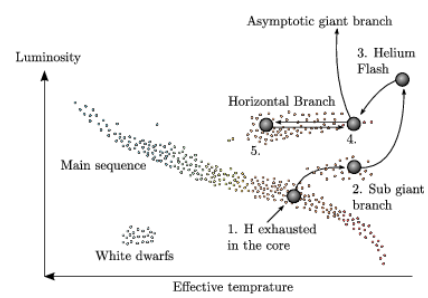
\includegraphics[scale = .5]{figures/horizontal_branch}
  \caption{HR-Diagram showing evolution of a star moving from main sequence to the horizontal branch}
  \label{fig: Main to giant}
\end{figure}  

\subsection{The End}
As our star experiences expansion and contraction multiple times as it oscillates between helium flashes it will lose more and more of its helium. In the end, the only thing left is an electron degenerate core of carbon and oxygen. It has now entered its final stage of life. It will live and die as a white dwarf becoming colder and colder through radiation as there is no more energy production. While its temperature is still relatively high, its luminosity is now very low and it will live the rest of its life in the bottom left corner of the HR-Diagram as seen in Figure \ref{fig: HR_diagram}. 

\subsubsection*{Mass}
Our star has a mass $ M < 8M_{⊙} $. We will therefore assume its mass as a white dwarf $ M_{\text{WD}} $ will obey the following equation. 
\begin{equation}\label{eq: Dwarf mass }
  M_{\text{WD}} = \frac{M}{8M_{⊙}} M_{\text{Chandresekhar}}
\end{equation}   
where $ M_{\text{Chandresekhar}} = 1.4 M_{⊙} $. 
Using our current mass we get a mass $ M_{\text{WD}} $ of
\begin{equation}\label{eq: Dwarf mass calculated }
  M_{\text{WD}} = 1.55 ⋅ 10_{30} \text{ kg} = 0.78 M_{⊙}
\end{equation}

\subsubsection*{Radius}
We want to find an expression of how large our star will become as a white dwarf. To do this we are going to assume the following. 
\begin{itemize}
  \item Hydrostatic equilibrium
  \item Uniform density
\end{itemize}

We can use the equation for hydrostatic equilibrium as derived in%~\parencite[][equation 1]{for_notat_3e}. TODO: Remove Comment
\begin{equation}\label{eq: Hydro equilibrium }
  \frac{P}{R} ≈  \frac{GM}{R^{2}} \frac{4M}{3 π R^{3}} = \frac{3GM^{2}}{4 π R^{5}}
\end{equation}
Replacing the pressure $ P $ with the degeneration pressure we get the equation from%~\parencite[][equation 2]{for_notat_3e}. TODO: Remove Comment
\begin{equation}\label{}
  \left( \frac{3}{π} \right) ^{\frac{2}{3}} \frac{h^{2}}{20m_e} n_{e}^{\frac{5}{3}} = \frac{3GM^{2}}{4 π R^{5}}
\end{equation}
where $ n_e $ is the electron number density which we can be rewritten using the total gas density as. 
\[
n_e = n_p = \frac{ρ_{\text{p}}}{m_{H}} = \frac{Z}{A} \frac{ρ}{m_{H}}
\]
where Z is the number of protons per nucleus and A is the number of nucleons per nucleus. We replace the density $ ρ $ with $ \frac{M}{V} $. As we assume the gas to be neutral there should be one neutron for every proton meaning $ \frac{Z}{A} = \frac{1}{2} $. Inserting this to equation \ref{eq: Hydro equilibrium } and solving for $ R $ we get an expression of the radius of our star as a white dwarf $ R_{\text{WD}} $. 
\begin{equation}\label{eq: Dwarf radius}
  R_{\text{WD}} ≈ \left( \frac{3}{2 π} \right) ^{\frac{3}{4}} \frac{h^{2}}{20 m_e G} \left( \frac{1}{2m_{H}} \right) ^{\frac{5}{3}} M_{WD} ^{-\frac{1}{3}}
\end{equation}
where $ m_e $ is the mass of an electron, $ m_h $ the mass of a proton and $ M_{\text{WD}} $ is the mass of our white dwarf. Using the mass we calculated in equation \ref{eq: Dwarf mass calculated } we get a radius $ R_{\text{WD}} $ 
\begin{equation}\label{eq: Darf radius calculated}
  R_{\text{WD}} = 1.55 ⋅ 10^{6}\ m 
\end{equation}
which is at the same order of magnitude as the planet Terra. 

\subsubsection*{Fun Facts}
We know that 1L of water weighs around 1kg. Lets try and see how much 1L of our white dwarf weighs! As we know its weigh and radius we can find its density $ ρ_{D}  = \frac{M}{V} = 9.82 ⋅ 10^{10} \frac{\text{kg}}{\text{m}^{3}}$. As one litre is $ 1 \text{dm}^{3} $ we just divide by 1000 and get at mass of 9.82 $ ⋅ 10^{7} $kg. Now that is heavy!

Ever wondered what it would be like to walk on a neutron star? Of course you have, but lets see if it is even possible. Using Newtons universal law of gravitation we get the following expression for the acceleration you would feel on its surface. 
\begin{equation}\label{eq: Dwarf gravity}
  a_D = G \frac{M_\text{WD}}{R^{2}} = 4.27 ⋅ 10^{7} \ \frac{\text{m}}{\text{s}^{2}}
\end{equation}
It does not seem likely there will be any walking on the neutron star after all. That is a lot of force pulling oneself down to the ground, but now you know!
  
\newpage
\phantom
\newpage
\newpage
\onecolumngrid
\section{Appendix} \label{sec: appendix}
\subsection{Detailed HR-Diagram}
\begin{figure}[h!]
  \centering
  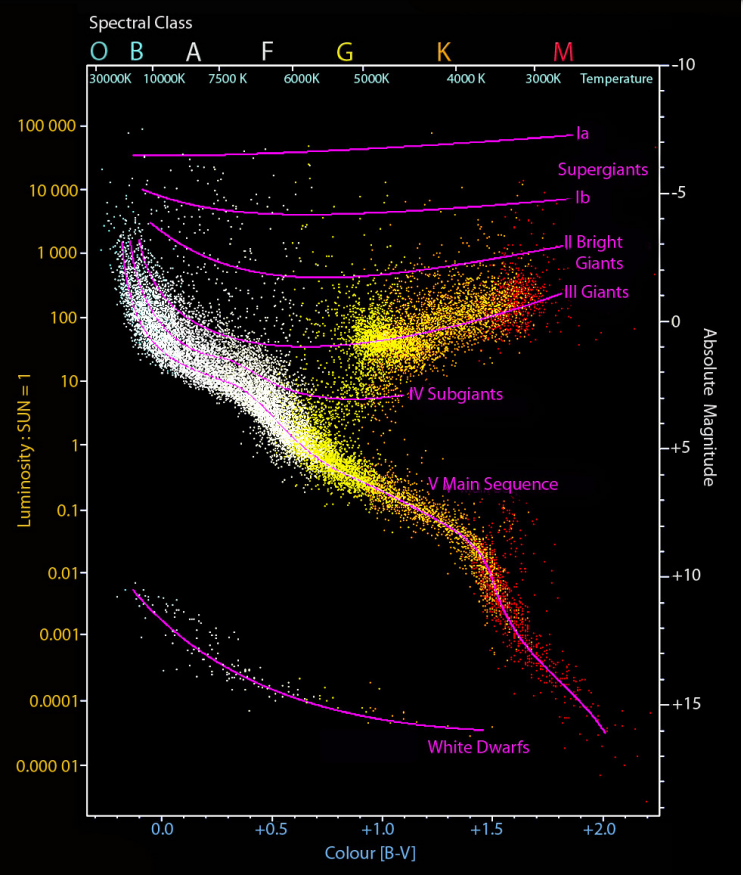
\includegraphics[scale = .75]{figures/Spectral_class}
  \caption{HR-Diagram showing different categorizations of stars%~\parencite[][page 2]{for_notat_3d}. TODO Remove Comment
  }
  \label{fig: Spectral class}
\end{figure}
\clearpage
\twocolumngrid

\newpage
%\printbibliography TODO: Remove Comment

\end{document}